\chapter{\ac{lora} \ac{phy} Testing}
\section{Overview}
It has been repeatedly shown that \ac{lora} transmissions can be received at distances exceeding 10km in  unobstructed environments (free-space) when antennas are highly elevated \cite{3YP:LORA_RANGE_REVIEW}. However, these ideal radio conditions are not realistic for swarm robots operating in high-propagation environments such as forests. Therefore the first experiment in this paper attempts to identify the physical performance of \ac{lora} for the sparse swarm use case. 

\chapter{Testing  Platform}\label{sec:testing_platform}
\section{Hardware}
The basis of the designed test platform is HopeRF's\footnote{HopeRF Microelectronics Co. Ltd, China, https://www.hoperf.com/} RFM95W - a packet radio containing a \ac{lora} transceiver design licensed from Semtech; specifically, a broken out version from  Adafruit's\footnote{Adafruit, USA, https://www.adafruit.com/} is used. As a raw packet radio it provides direct access to the radio interface. An omni-directional 3dBi gain half-wavelength whip antenna is connected to the radio using a soldered uFL connector and a SMA to uFL connector. The net gain is assumed to be approximately 0dBm, after accounting for 1.5dBm loss in the cable (datasheet), 0.5dBm lost in the uFL connector (datasheet) and 1dBm lost through soldering (estimate). It is controlled by a Teensy\footnote{Teensy, https://www.pjrc.com/teensy/} 3.6 micro-controller, which also handles all logging responsibilities. A simple breakout circuit is implemented on strip-board to connect the components in a condensed package. Each breakout board features: a JST-PH2 battery connector, a coin cell holder for the Teensy's real-time-clock (\ac{rtc}), a power switch, a two-mode software switch, and three status LEDs. The schematic can be viewed in Figure \ref{fig:datalogger_schematic}. This is packaged to fit in an IP67 rated container with an internal lithium-polymer battery. Switches and SMA antenna connectors are external; these are IP67 rated and sealant is added where appropriate. The Teensy is equipped with an SD card for storage but, due to cost considerations, a GPS module is not implemented. A full breakdown of materials is listed in Figure \ref{fig:datalogger_cost}. The created test platforms, seen in Figure \ref{fig:dataloggers}, achieve the target of being a \ac{lora} datalogger suitable for all-weather.

\begin{figure}[H]
    \centering
    \begin{tabular}{cc}
    \subfloat[]{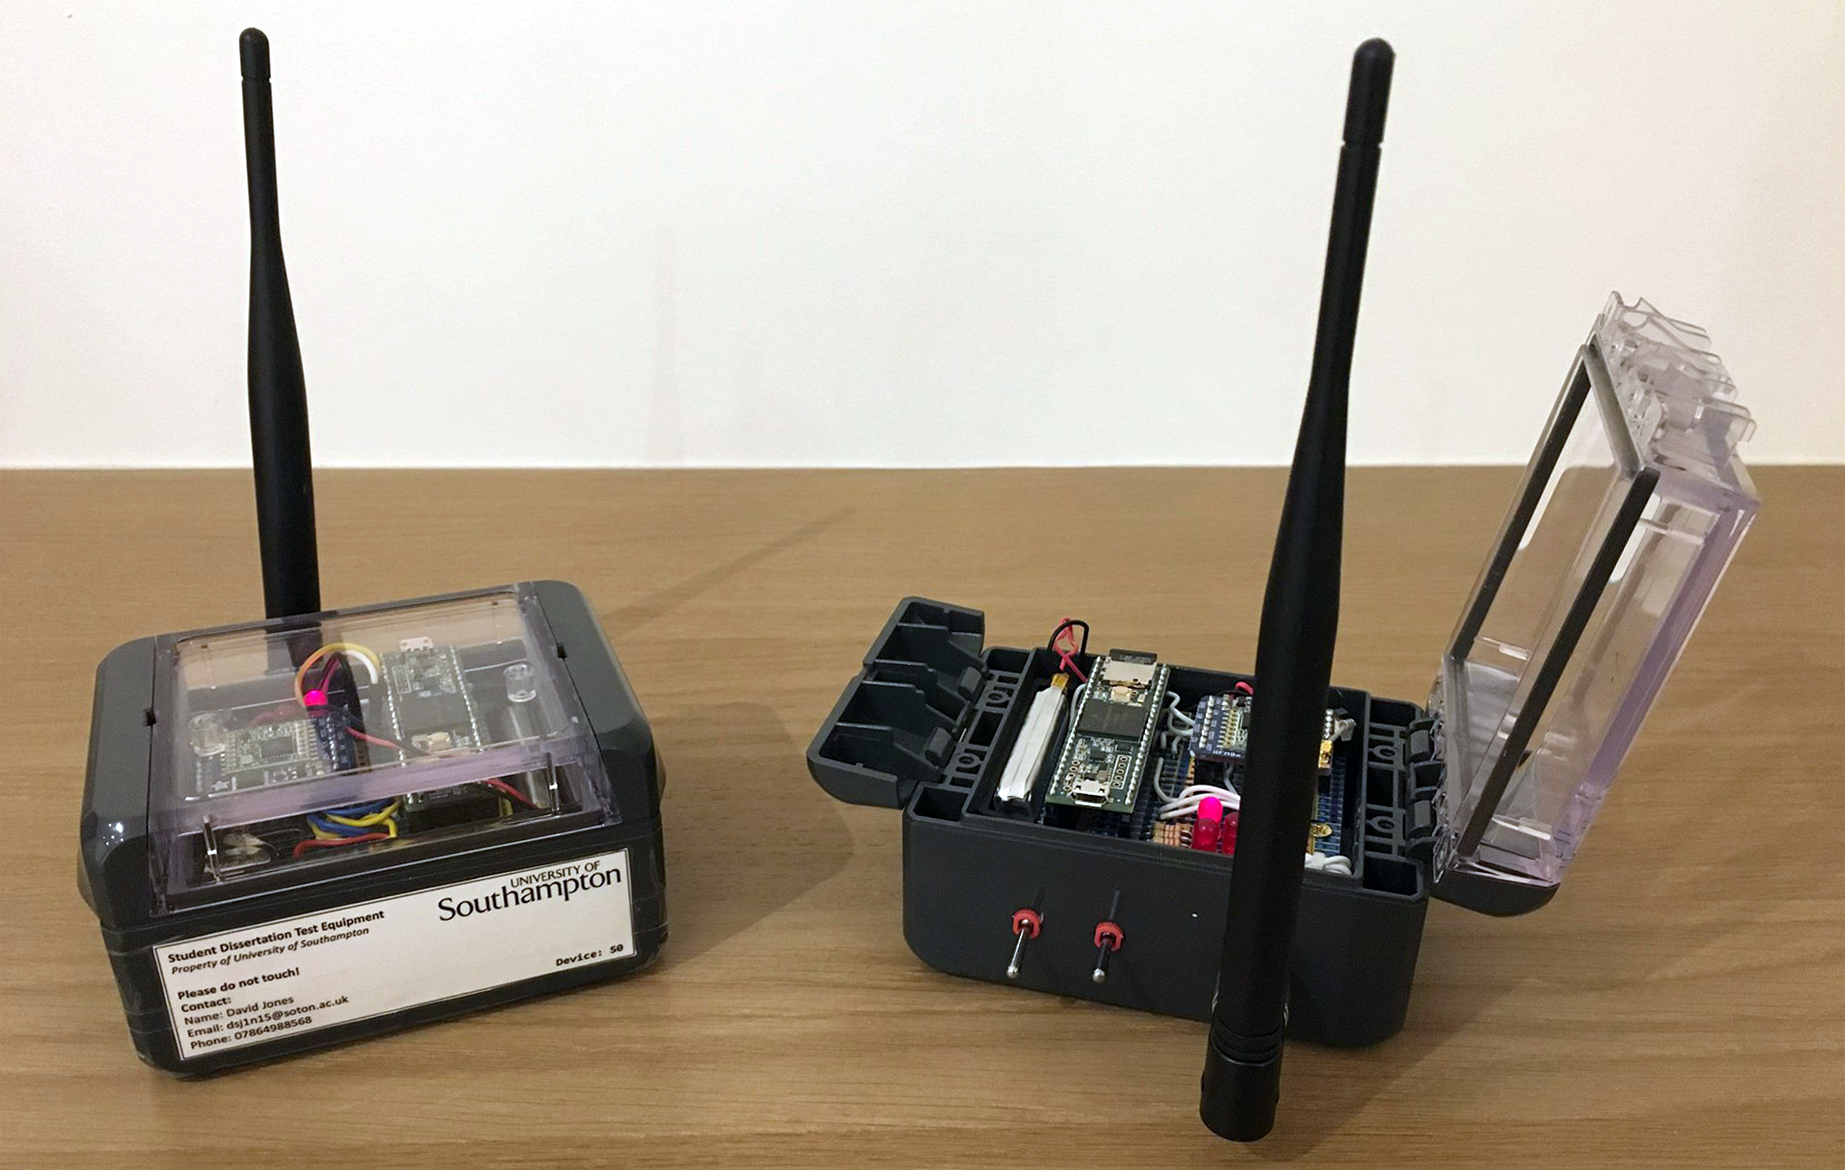
\includegraphics[height=5cm]{Figures/dl_both_devices.png}}
    \hspace{2.5mm}
    \subfloat[]{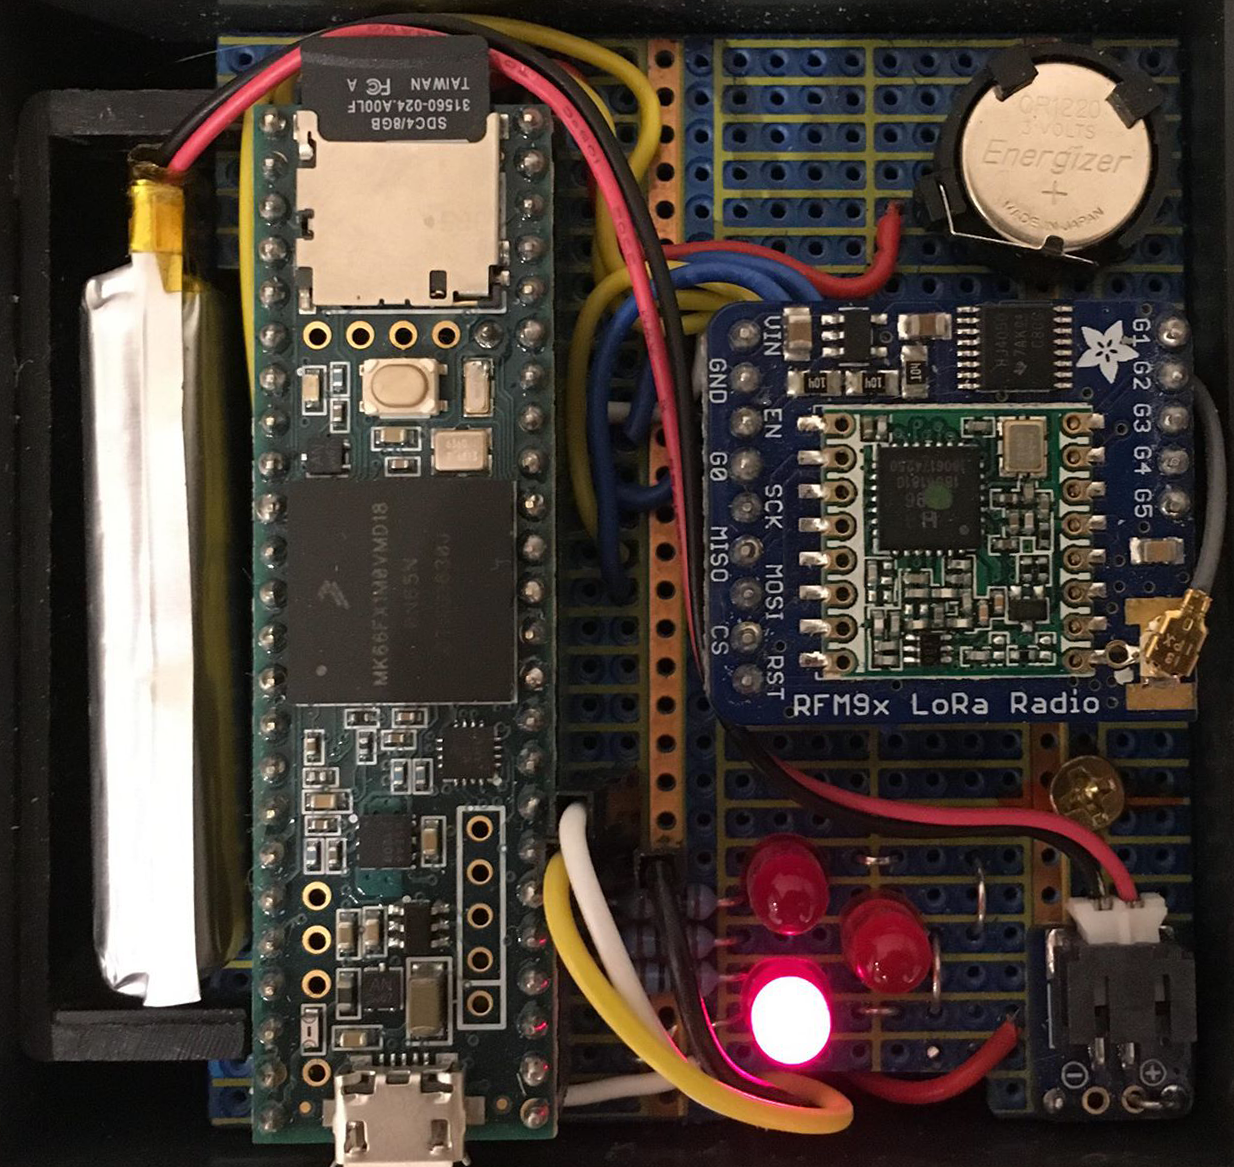
\includegraphics[height=5cm]{Figures/dl_circuit.png}}
    \end{tabular}
    \caption[Assembled testing platform]{External view of \texttt{S0} and \texttt{M0} platforms (left). Circuit view of \texttt{S0} (right); this is fixed into the assembly to avoid movement between tests. }
    \label{fig:dataloggers}
\end{figure}

\section{Software}\label{sec:test_platform_software}
The system is designed such that one device (a slave), can be left unattended at a fixed location and controlled by a second device (a master); this is achieved using a command control system, as explained in Figure \ref{fig:software_cmd_system}. Two command classes are defined for testing purposes; these are as follows:
\begin{itemize}
\vspace{-5mm}
	\item {\textbf{\texttt{HB\_CMD}}} : Command to trigger simple heartbeat functionality. When a slave receives this command it sends a heartbeat response (\textbf{\texttt{HB\_RSP}}) on the base configuration.
	\item {\textbf{\texttt{TD\_CMD}}} : Command to trigger execution of a test definition (\ac{td}). A \ac{td} holds a \ac{lora} configuration (values for \ac{cf}, \ac{sf}, \ac{tp}, \ac{bw}, \ac{cr}, \ac{pl}), a required \ac{pc}, and packet length. Figure \ref{fig:software_testdef_execution} explains the full control flow in detail.
	\end{itemize}
	
Slaves always listen to handle incoming commands, whereas the master can be set into two modes:
\vspace{-5mm}
\begin{itemize}
	\item \textbf{Heartbeat:} Sends periodic \texttt{HB\_CMD} commands, alerts user accordingly for every received or missed \textbf{\texttt{HB\_RSP}}.
	\item {\textbf{Run \ac{td}s:} Loads all stored \ac{td}s and handles them sequentially using \textbf{\texttt{TD\_CMD}}s.}
\end{itemize}
Interfacing with the radio is handled by the RH\_RF95 driver from the Radiohead\footnote{Radiohead, https://www.airspayce.com/mikem/arduino/RadioHead/} library. Operation of the software is detailed in Appendix \ref{sec:user_manual}.

\begin{figure}[p]
    \centering
    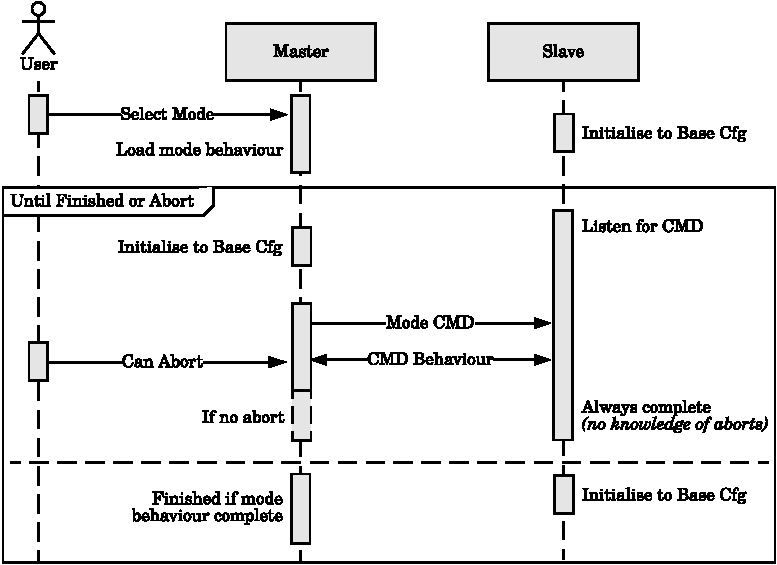
\includegraphics{Figures/software_cmd_system}
    \caption[Master-Slave command control method]{
    	Diagram showing master-slave command control method. Initially, both devices default to the same hardcoded radio parameters allowing two-way communication. This base state is chosen such that the expected range exceeds or matches that of the longest test range. When a mode is selected on the master, it sends the corresponding command to the listening slave and the behaviour is carried out. At any point the user may stop the master, and unless the slave is interacting with the master, it likely has no knowledge of this and will finish its behaviour. After command behaviour has finished the base configuration is reloaded in case it has been changed. In the case a master's mode requires multiple commands, the process repeats.
    }
    \label{fig:software_cmd_system}
\end{figure}
\begin{figure}[p]
    \centering
    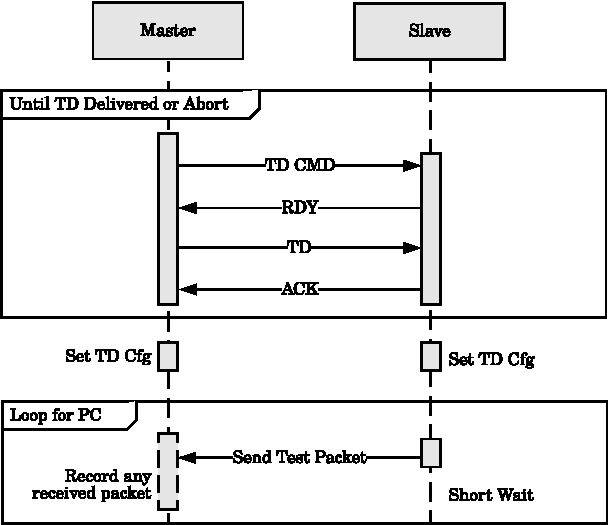
\includegraphics{Figures/software_testdef_execution}
    \caption[Master-Slave test definition execution method]{
    	Diagram showing execution of a single \ac{td}. After a \textbf{\texttt{TD\_CMD}} command is received, a short handshake takes place so that the master can share the \ac{td} to execute. After which both radios accordingly change their parameters and the slave sends the required \ac{pc}. Test packets are of length defined by the \ac{td} and contain a sequence identifier with the rest of data filled by a fixed data pattern. Any received packets are recorded along with \ac{rssi} and \ac{snr} values. Failed receives that occur due to bad CRCs are also recorded. This means that only transmissions where the preamble is not received are not recorded.
    }
    \label{fig:software_testdef_execution}
\end{figure}

\section{Methodology}
Simple testing scenarios devised.
so a phone was used for logging test coordinates manually

\section{Results}
\the\textwidth
\begin{figure}[H]
    \centering
   	\includegraphics{Figures/snr_pp_plot.eps}
    \caption[\ac{snr} vs packet percentage plot]{
    WRITE THIS DESCRIPTIONNN!!!
    }
    \label{master_slave_sequence}
\end{figure}

\subsection{Open (Free) Space}
High noise floor indicates that either the receiver's noise figure is not correct or there is more noise than expected in the environment. The fact that demodulation limit is nowhere near the true limit for SF10 onwards suggests that the cheaper radio does not perform correctly.


\subsection{Forest}
\subsection{Radio Height}

% Testing platform
% Testing methodology 
% Distance in relatively open space (got)
% Distance in trees (got)
% Closeness to ground (got)
% Coding rate ??? (sort of got)
% Difference in slight movements (!!!)
%Lessons Learnt 
https://www.thethingsnetwork.org/forum/t/no-lower-rssi-than-121-dbm-possible-in-ttn/19890/15